\chapter{Koncepcja}

W rozdziale omówiona zostanie koncepcja i zasada działania inteligentnej kamery. 

\section{Maksymalizacja szybkości}
 
Szybkość działania kamery jest jednym z kluczowych założeń działania systemu. W zależności od przeznaczenia systemu może się znacznie różnić. W dziedzinach wyspecjalizowanych, takich jak robotyka, czy TODO
\begin{description}
\item Czynniki składające się na ogólną szybkość działania kamery:
	\begin{enumerate}[noitemsep]
	\item Przetwarzanie obrazu przez sensor oraz protokół komunikacyjny między sensorem, a płytą.
Według danych producenta czas potrzebny na wygenerowanie jednej klatki wynosi ok 1/90 s dla rozdzielczości strumienia 640x480. Protokół zastosowany w kamerze, to Camera Serial Interface wykorzystujący 2 linie danych umożliwiających maksymalną prędkość przesyłu na poziomie 2Gbps (1Gbps na linię).
\item Przetwarzanie obrazu przez sterownik obrazu (kompresja danych).
Czas ten jest uwarunkowany wydajnością akceleratora graficznego i  ze względu na wydajną jednostkę GPU VideoCore IV uznawany jest w projekcie za pomijalny.
\item Przetwarzanie danych przez aplikację.
Głównym czynnikiem mającym wpływ na ten czas jest algorytm zastosowany do detekcji twarzy. Dokładny jego opis znajduje się w rozdziale 3.6.1
\item Szybkość przesyłu danych przez interfejs Ethernet
Protokół Ethernet jest jednym z podstawowych interfejsów komunikacji urządzeń w lokalnych sieciach komputerowych. Zastosowana w płycie Raspberry Pi 2 wbudowana karta sieciowa wg informacji producenta umożliwia transfer danych z przepustowością 10 lub 100 Mb/s.
		\end{enumerate}
\end{description}

Ważnym aspektem są czas odpowiedzi systemu dla każdej z ww. operacji oraz ogólne czasy odpowiednio między wykryciem twarzy a : \\
-akcją sprzętową (np. otwarciem drzwi, włączeniem alarmu)\\
-umieszczeniem logu na serwerze.\\
W projekcie przyjęto założenie, że w celu poprawy skuteczności detekcji obiektu minimalny czas między zdarzeniem wykrycia obiektu określony będzie przez użytkownika. Rozdział  4. aspekt ten opisuje dokładniej.

\section{Inteligencja dostosowana do wymogów monitoringu}
Inteligentny system monitorujący wymaga, aby oprócz dostarczania obrazu dokonać także jego przetworzenia – tj. za pomocą odpowiednich algorytmów dokonać detekcji żądanych obiektów.
Podrozdział 3.6.1 traktuje szczegółowo o tym zagadnieniu.

\section{Modularność }

\begin{description}
\item Struktura modularna pozwala zapewnić dużą kontrolę przy projektowaniu i debugowaniu działania aplikacji. Aplikacja jest pisana zgodnie z techniką programowania obiektowo orientowanego (w skrócie OO), wyróżnić można kolejne kroki :
\begin{enumerate}[noitemsep]
\item Rozpoznanie problemu. \\%enter
Przeprowadzona została analiza funkcjonalności systemu i wymagań, zgodnie z założeniami z rozdziału 3.1.
\item Projektowanie programu. \\
Na ten etap składa się : zidentyfikowanie zachowań systemu i obiektów w nim występujących, a następnie określenie ich hierarchii ( dziedziczenie ) i sekwencji działania.



Obiekty występujące w systemie to :
\begin{itemize}[noitemsep]
\item Module – bazowa klasa abstrakcyjna
\item Object Detect – klasa implementująca detekcję obiektów
\item Worker – klasa odpowiedzialna za wszelkiego rodzaju akcje
\item Logger – klasa implementująca mechanizm generowania logów. Współpracuje bezpośrednio z Object Detect
\item Controller – główna klasa zarządzająca pozostałymi, implementuje „logikę” kamery.
\end{itemize}

Do konkretnych zachowań można zaliczyć : detekcję obiektów, wykonanie akcji (sterowanie portami GPIO), stworzenie pliku logów. Każda z wymienionych klas dziedziczy po Module.
Sekwencja działania jest zdefiniowana następująco :
\begin{enumerate}[noitemsep]
\item Object Detect po wykryciu twarzy, wysyła sygnał do Controllera
\item Controller ustawia flagę detected=true, odczekuje ustalony przez użytkownika czas \textbf{latency }
\item Jeśli po upływie \textbf{latency} Controller otrzyma ponownie sygnał, to zleca modułowi Worker i Logger pracę - wykonanie akcji sprzętowej i wygenerowanie pliku z logiem.
\item Po wykonaniu pracy Worker wysyła do Controllera sygnał
\item Po odebraniu sygnału od Worker’a Controller zatrzymuje pracę modułu Object Detect
\item Po wykryciu zamkniętych drzwi Worker wysyła sygnał do Controllera
\item Odebranie sygnału od Workera powoduje wznowienie pracy Object Detect
\end{enumerate}
\item Implementacja: \\
Implementacja komunikacji między obiektami zrealizowana jest z wykorzystaniem mechanizmu sygnałów biblioteki Boost. Daje to możliwość przekazania sterowania danemu obiektowi poprzez wywołanie funkcji obiektu zlecanego - zbindowanej w slocie wraz z przekazanym argumentem określonego typu.
\item Testowanie: \\
Ważnym aspektem poprawnej pracy systemu są testy. System musi spełniać nie tylko warunek poprawnego działania, ale też spełniać wymagania czasowe. Rozbieżności takie mogą w konsekwencji prowadzić do trudnych do wykrycia awarii, niekoniecznie urządzenia kamery ale np. urządzenia sterowanego, czy też powodować zakłamania w wynikach pracy kamery.
Argumentem dla wyboru techniki OO jest fakt, iż system w przyszłości może realizować inne zadania/warunki, w konsekwencji aplikacja będzie potencjalnie modyfikowana i sukcesywnie rozbudowywana.
\end{enumerate}
\end{description}

\section{Interface użytkownika}
Jako interfejs użytkownika służy serwer http – Apache 2. Na podstawie dostarczonych od modułu Logger  zdjęć generuje odpowiednie wpisy i umieszcza je na stronie WWW. Za generację logów po stronie serwera odpowiedzialne są skrypty napisane z wykorzystaniem technologii PHP i jQuery.

Dane takie jak data, godzina są zawarte w nazwie plików, natomiast zostaną wyodrębnione przez ww. skrypty. Strona WWW odświeżana jest automatycznie  co 1s.  Szczegółowy opis działania skryptów opisany jest w podrozdziale 3.6.3.

\section{Funkcje systemu}

%Funkcje systemu :
\begin{itemize}[noitemsep]
\item Detekcja obiektów \\
Obiekty te mogą być w zasadzie dowolnego typu. Detekcja opiera się na wytrenowaniu algorytmu dlatego mogą to być zarówno obiekty rzeczywiste, takie jak: twarze ludzkie, litery, pojazdy itp., oraz specyficzne wzory pozwalające identyfikować jednoznacznie żądane obiekty.

\item Sterowanie modułem zewnętrznym \\
W zależności od wymagań mogą to być: manipulatory robotów, sterowniki bram, napędy, czujniki, a także inne aplikacje, które oczekują na informacje od kamery ( np. ilość obiektów i ich czasy poruszania się, czy też orientacja w przestrzeni).

\item Logowanie zdarzeń na serwerze http \\
Dzięki interfejsowi Ethernet możliwa jest komunikacja systemu z użytkownikiem. Np. umieszczanie na serwerze logów, lub danych przetworzonych przez urządzenie w bazie danych. 

\item GUI \\ 
Dodatkową funkcjonalnością przewidywaną przy dalszej rozbudowie systemu jest graficzny interfejs użytkownika GUI (ang. Graphic User Interface), pozwalający na szybszą i  bardziej intuicyjną interakcję użytkownika z systemem.

\item Sterowanie zewnętrznymi akcjami \\
W projekcie kamera łączy role systemu monitoringu i sterownika drzwi:  ma za zadanie wykryć twarze osób, które pojawią się przed drzwiami, a następnie je otworzyć. Kolejnym krokiem jest umieszczenie  na serwerze logu w postaci : zdjęcia danej osoby oraz daty i godziny pojawienia się. Dostęp do logów będzie możliwy dla każdego użytkownika posiadającego urządzenie posiadające przeglądarkę stron WWW ( czyli smartfony, tablety, komputery itd.) i będące w obrębie sieci, w której pracuje kamera.
Ogólna idea zastosowania kamery jest zilustrowana na rysunku 3.1.
\end{itemize}

\begin{figure}[bth]
\centering
{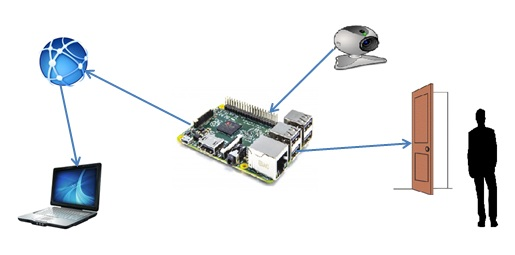
\includegraphics[width=1\linewidth]{sch/Koncepcja_ogolna_projektu}}
\caption[Koncepcja ogólna projektu]{Koncepcja ogólna projektu}
\label{fig:sch2}
\end{figure}

\section{Szczegółowe omówienie funkcji}
\subsection{Detekcja obiektów}
Do realizacji detekcji obiektów wykorzystana zostanie biblioteka OpenCV (Open Computer Vision). Bibliotekę tę cechuje wieloplatformowość, kilka interfejsów programistycznych, modularna struktura oraz wiele algorytmów z zakresu wizji komputerowej i uczenia maszynowego. 

W projekcie użyty został interfejs C++, natomiast platformą docelową jest Linux w dystrybucji Raspbian.

Detekcja obiektów jest zaawansowanym zagadnieniem wizji komputerowej. Biblioteka OpenCV dostarcza wiele funkcji umożliwiających łatwe użycie algorytmów. Poniżej zamieszczony jest opis działania  algorytmu detekcji obiektów Viola-Jones.
 
\paragraph{Cechy algorytmu Haara.} Główną ideą działania algorytmu jest wykorzystanie przesuwnego, skalowalnego okna, które posiada tzw.  cechy Haara (ang. Haar features). 

Cechy te nakładane są na dany obraz w celu określenia przynależności danego obszaru do klasy obiektów poszukiwanych. Dla każdej cechy obliczana jest różnica sumy wartości pikseli znajdujących się na obszarach białych i czarnych.

\begin{figure}[bth]
\centering
{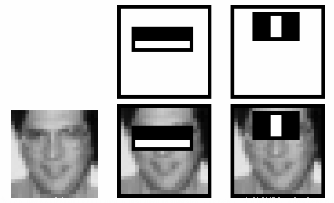
\includegraphics[height=0.35\linewidth]{sch/haar}}
{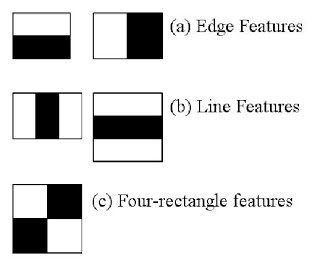
\includegraphics[height=0.35\linewidth]{sch/haar_features}} \\
\caption[ Cechy Haara i wykorzystanie cech Haara do detekcji twarzy.]{Cechy Haara i wykorzystanie cech Haara do detekcji twarzy.}
\label{fig:sch2}
\end{figure}

Uwzględniając wszystkie możliwe wymiary i położenia dla okna przesuwnego np. o wymiarach 24x24, liczba cech wynosi ponad 160 000. Ograniczone zasoby sprzętowe standardowych komputerów klasy PC, a tym bardziej systemów wbudowanych nie pozwalają na wykonanie tej skali obliczeń w sensownym czasie. Dlatego podstawową ideą jest wyeliminowanie ze zbioru cech, tych które są nieistotne w procesie detekcji. Tutaj z pomocą przychodzą obrazy całkowe(ang. Integral images) i algorytm AdaBoost (Adaptive Boosting).

\paragraph{Obrazy całkowe}
Pozwalają one na szybkie i efektywne obliczanie sumy wartości pixeli w określonym obszarze cechy.

Metoda ta wykorzystuje zależność, która pozwala obliczyć wartość sumy pixeli z obszaru ograniczonego przez zaledwie cztery punkty A=(x0,y0),B=(x1,y0),C=(x0,y1),D=(x1,y1) 

$$ \sum_{\binom{x0<x<x1}{y0<y<y1}} i(x,y) = I(D) + I(A) -I(B) - I(C)$$
gdzie:
$$ I(x,y) = \sum_{\binom{x'<x}{y'<y}}$$

Co zilustrowano na rysunku \ref{fig:sch2}.
\begin{figure}[bth]
\centering
{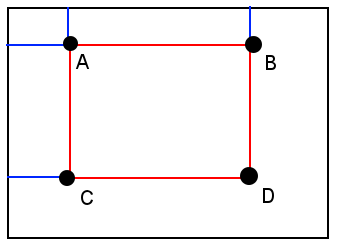
\includegraphics[height=0.35\linewidth]{sch/pxel}}
\caption[ Obliczanie sumy wartości pixeli fragmentu obrazu]{Obliczanie sumy wartości pixeli fragmentu obrazu.}
\label{fig:sch2}
\end{figure}




\paragraph{Algorytm AdaBoost} opracowany i zaprezentowany w 1997 r. przez Yoava Freunda i Roberta Schapire jest jednym z wielu realizujących tzw. boosting. W wyniku procesu uczenia algorytmu otrzymujemy silny klasyfikator binarny, który składa się ze słabszych klasyfikatorów z odpowiednimi wagami. Klasyfikator taki daje nam jednoznaczną informację czy dany obiekt należy do klasy poszukiwanych, czy też nie. Budowany jest w procesie uczenia, gdzie na wejście podaje się tzw. zestaw treningowy (ang. training set), a na wyjściu otrzymujemy gotowy klasyfikator zdolny do pracy z nowym zbiorem danych.
Klasyfikator słaby, to taki, którego błąd klasyfikacji jest mniejszy niż 0.5, czyli lepszy niż zwykłe zgadywanie.

Opis algorytmu:
%Algorytm AdaBoost
Wejście: zbiór przykładowych obrazów $(x_1,y_1),..,(x_n,y_n)$, gdzie $y_i=0,1$ dla odpowiednio negatywnych i pozytywnych próbek.
Wyjście: silny klasyfikator $H(x)$.
Kroki algorytmu :
\begin{enumerate}
\item Dla każdego z k elementów zestawu trenującego T  przypisz identyczną wagę początkową.
$$W^1(i)= \frac{1}{k}  , i = \{1,...,k\} $$
Liczba iteracji wynosi $N$.
\item Dla $n=1,…,N$: 
Wybierz słaby klasyfikator o najmniejszym błędzie $\epsilon_n$
	$$\epsilon_n = \sum_i W_i |h_n(x_i)-y_i	| $$
\item Oblicz nową wagę 
$$\alpha_n = \frac{1}{2} ln \frac{1-\epsilon_n}{\epsilon_n}$$  
\item Dla poprawnie sklasyfikowanych przykładów trenujących xi wagi są uaktualniane na podstawie zależności:
$$W_{n+1} = \frac{W_n(i)exp(-\alpha n)}{z}$$
Dla niepoprawnie sklasyfikowanych przykładów :
$$W_{n+1} = \frac{W_n(i)exp(\alpha n)}{z}$$
gdzie Z- stały czynnik normalizujący.
 
\item Klasyfikator końcowy:
 $$H(x) =\begin{cases}1 \sum^N_{n=1} \alpha_n h_n(x) \geq \frac{1}{2} \sum^N_{n=1} \alpha \\
 0 \end{cases} $$
\end{enumerate} 

Podsumowując AdaBoost wykorzystuje te cechy, które są w stanie wykryć samodzielnie więcej niż połowe przypadków. Poprzez zmniejszanie wag cech poprawnie wykrywających obiekty i zwiększanie wag  cech, które sklasyfikowały obiekty błędnie, algorytm	 potrafi „skupić się” na trudnych przypadkach.	
Klasyfikator zaproponowany przez autorów biblioteki OpenCV zawiera po wytrenowaniu około 6000 cech. Jest to ogromna redukcja względem wspomnianych 160 000,  jednakże wciąż zbyt dużo, aby zapewnić detekcję obiektu w krótkim czasie. Rozwiązaniem jest kaskada klasyfikatorów.
\paragraph{Kaskada klasyfikatorów}

Większość z obszaru analizowanych obrazów nie zawiera twarzy. Stąd wyszedł pomysł,  aby ocenić czy obszar może zawierać twarz już na samym początku. Jeśli nie, odrzucić ten region, a skupić się na tych, które faktycznie mogą zawierać twarz. Taki zabieg pozwala oszczędzić mnóstwo czasu i zasobów sprzętowych.
Zamiast sprawdzać wszystkie 6000 cech autorzy proponują podzielić proces detekcji na wiele etapów. W każdym z etapów są zgrupowane określone cechy nakładane jedna po drugiej, przy czym ilość cech sprawdzanych w kolejnych etapach rośnie. Jeśli obraz nie przejdzie początkowych etapów jest odrzucany i sprawdzany jest kolejny. Natomiast jeśli przejdzie wszystkie etapy – klasyfikowany jest jako twarz. Zasadę działania kaskady ilustruje rysunek \ref{fig:kaskada}.

\begin{figure}[bth]
\centering
{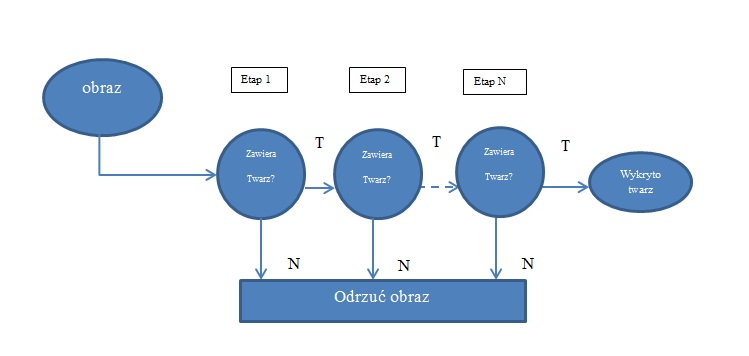
\includegraphics[width=1\linewidth]{sch/kaskada}}
\caption[Kaskada klasyfikatorów dla N etapów.]{Kaskada klasyfikatorów dla N etapów.}
\label{fig:kaskada}
\end{figure}

Biblioteka OpenCV w pakiecie zawiera także narzędzia, które pozwalają samemu wytrenować klasyfikator zdolny do rozpoznania dowolnych obiektów. Aby jednak wytrenować dość silny klasyfikator potrzeba dużej ilości pozytywnych i negatywnych przykładów. Stąd też zdecydowano się użyć dostarczonych w pakiecie biblioteki gotowych klasyfikatorów. Proces trenowania przedstawiony jest na schemacie \ref{fig:trening}. W wyniku działania narzędzia HaarTraining otrzymujemy plik XML ze zdefiniowanym klasyfikatorem, gotowym do użycia w aplikacji.

\begin{figure}[bth]
\centering
{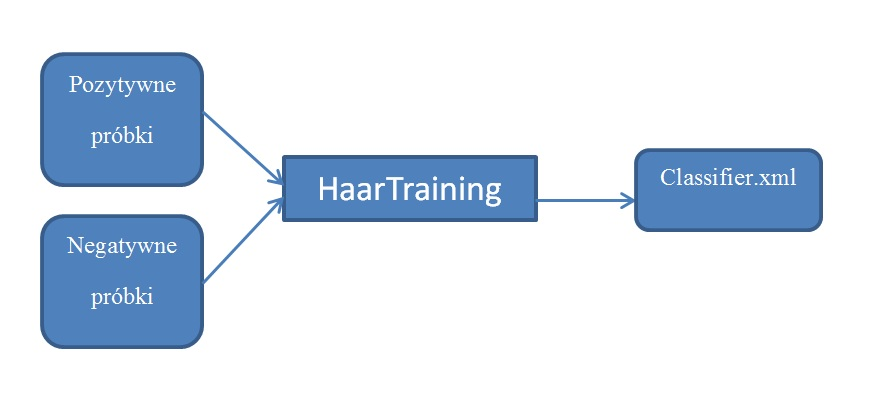
\includegraphics[width=1\linewidth]{sch/trening}}
\caption[Schemat trenowania klasyfikatora]{Schemat trenowania klasyfikatora}
\label{fig:trening}
\end{figure}

\subsection{ Sterowanie urządzeniem zewnętrznym}
Sterowanie urządzeniami zewnętrznymi zrealizowane jest przez programowe wystawianie stanów logicznych na portach GPIO płyty. Pozwala to po zestawieniu z układem sterowanym na kontrolę urządzeniem. W projekcie znajduje się implementacja, która pozwala na zaadaptowanie kamery do sterowania urządzeniem zewnętrznym. Sygnały cyfrowe można zastosować do dowolnego przeznaczenia np. włączenie alarmu, światła, klimatyzacji, powitania gościa...

 \begin{figure}[bth]
\centering
{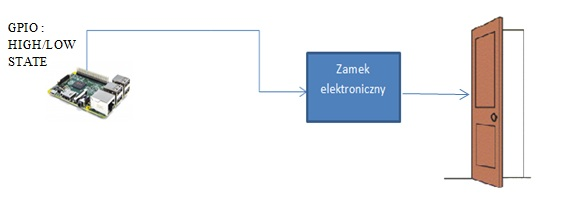
\includegraphics[width=1\linewidth]{sch/sterowanie}}
\caption[Koncepcja sterowania urządzeniem zewnętrznym]{Koncepcja sterowania urządzeniem zewnętrznym}
\label{fig:sterownie}
\end{figure}

\subsection{ Logowanie zdarzeń na serwerze HTTP}
Interfejs Ethernet zapewnia możliwość interakcji kamery z użytkownikiem.  Jej realizacja opiera się o serwer http, który  będzie wykonywał  skrypt napisany w technologii PHP i jQuery i wynik działania umieszczał na stronie internetowej.
Efektem czego użytkownik będzie mógł połączyć się z serwerem z dowolnego urządzenia, które posiada przeglądarkę stron WWW.  
\paragraph{Serwer http.}
Jako serwer wykorzystano Apache 2 – popularny, darmowy serwer http współpracujący z różnymi językami programowania oraz ze wsparciem dla baz danych – MySQL, PHP etc.
Współpracuje z systemami Linux, Windows i Mac OS. W projekcie uruchamiany jest na Linuxie.
 
 
\begin{figure}[bth]
\centering
{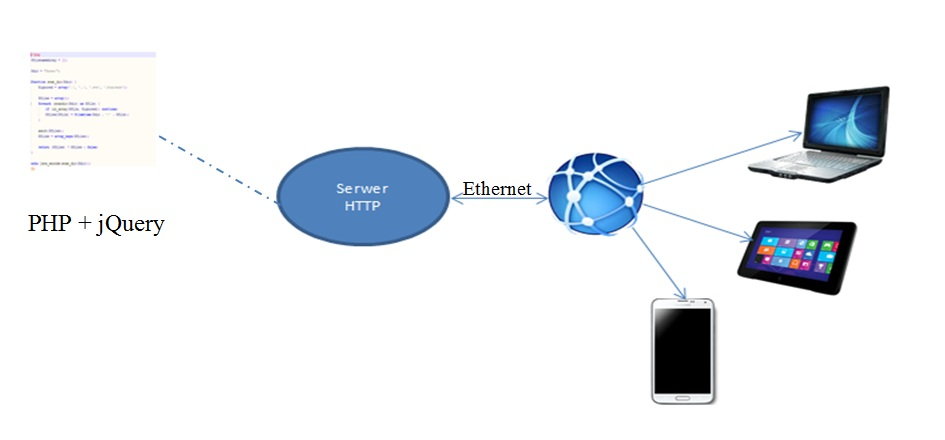
\includegraphics[width=1\linewidth]{sch/interface_komunikacji}}
\caption[Koncepcja interfejsu komunikacji z użytkownikiem]{Koncepcja interfejsu komunikacji z użytkownikiem}
\label{fig:komunikacja}
\end{figure}






